Fig.~\ref{fig:learning} shows the median relative error as a function of the number of training events for SIS and SIE+shear lenses (ET). The errors stop decreasing above $\sim10^4$ events. The results are therefore not limited by the size of the ET training sets (36\,000 events per family), while the O5 samples (900--1800 training events per family) lose about 1--2 percentage points relative to the asymptotic accuracy.

\begin{figure}
\centering
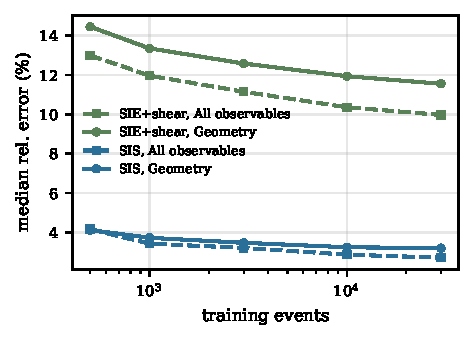
\includegraphics[width=\columnwidth]{fig_learning.pdf}
\caption{Median relative error of $\mu_A$ versus the number of training events for ET.}
\label{fig:learning}
\end{figure}
